\subsection{Asymmetric loss function} \label{supervised_approach_asymmetric}

In this section, we experiment with the \acrfull{asl} \cite{ben2020asymmetric}, which was already presented in section \ref{hmc_asl}. It extends the \acrfull{bce} loss to address the imbalance between positive and negative samples in multi-label settings. We experiment with the two parameters of \acrshort{asl}. We first test two different values for $\gamma_-$ while keeping the other constant, and then do the same the other way around. All other aspects of the model are those that worked best in the previous section: one-cycle learning rate policy, smaller hidden layer size and larger dropout rate.

\subsubsection{Negative gamma}

\begin{figure}
  \begin{subfigure}[t]{.5\textwidth}
    \centering
    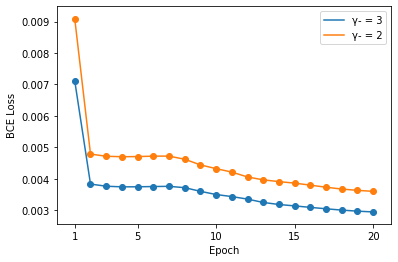
\includegraphics[width=\textwidth]{figures/supervised_approach/asl_neg_train_loss.png}
    \caption{Training loss}
    \label{fig:asl_neg_train_loss}
  \end{subfigure}
   \begin{subfigure}[t]{.5\textwidth}
    \centering
    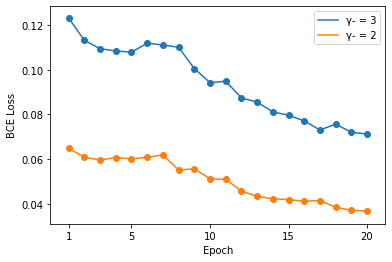
\includegraphics[width=\textwidth]{figures/supervised_approach/asl_neg_test_loss.png}
    \caption{Testing loss}
    \label{fig:asl_neg_test_loss}
  \end{subfigure}
  \caption{Test and training loss of models with different neg. gamma values.}
  \label{fig:asl_neg_train}
\end{figure}

\begin{figure}
  \begin{subfigure}[t]{.32\textwidth}
    \centering
    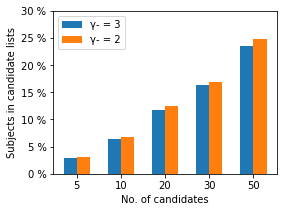
\includegraphics[width=\textwidth]{figures/supervised_approach/asl_neg_hw.png}
    \caption{Handwritten subjects}
    \label{fig:asl_neg_hw}
  \end{subfigure}
  \begin{subfigure}[t]{.32\textwidth}
    \centering
    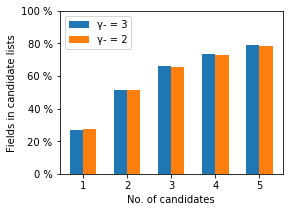
\includegraphics[width=\textwidth]{figures/supervised_approach/asl_neg_ddc.png}
    \caption{DDC subjects}
    \label{fig:asl_neg_ddc}
  \end{subfigure}
   \begin{subfigure}[t]{.32\textwidth}
    \centering
    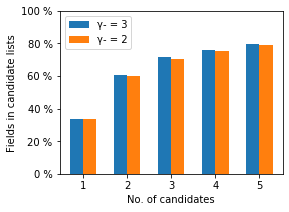
\includegraphics[width=\textwidth]{figures/supervised_approach/asl_neg_venue.png}
    \caption{Venues}
    \label{fig:asl_neg_venue}
  \end{subfigure}
  \caption{Model hit rate in the evaluation sets for different neg. gamma values.}
  \label{fig:asl_neg_eval}
\end{figure}

ASL improves the model training by reducing the importance of negative samples in the loss function, as they are much more numerous than positive samples, and they hinder the model from learning about the positive samples. Here we experiment with two values for $\gamma_-$: two and three. The authors usually set $\gamma_-=4$. If the first experiment favors $\gamma_-=3$, we will experiment with larger values for $\gamma_-$.

The model with $\gamma_-=3$ slightly outperforms the other model in the evaluation datasets that involve the assignment of fields, as can be seen in figures \ref{fig:asl_neg_ddc} and \ref{fig:asl_neg_venue}. On the other hand, the model with the lower $\gamma_-$ is better on the handwritten evaluation dataset, where subjects of deeper levels of the hierarchy are considered, as shown in figure \ref{fig:asl_neg_hw}.

Given that the difference in favor of the lower $\gamma_-$ on the handwritten evaluation dataset is larger than the difference against it on the other two datasets, where the difference is very small, we favor the lower $\gamma_-$ value. This means that decreasing the importance of negative samples too much hinders the learning process of the model.

Some differences in performance may arise from the random initialization of the models. As shown in figure \ref{fig:asl_neg_train}, the model trained with the lower $\gamma_-$ already started with a lower testing loss after the first epoch. However, the difference between the two models remains steady throughout the later epochs. We therefore don't believe it is necessary to repeat the experiment.

\subsubsection{Positive gamma}

\begin{figure}
  \begin{subfigure}[t]{.5\textwidth}
    \centering
    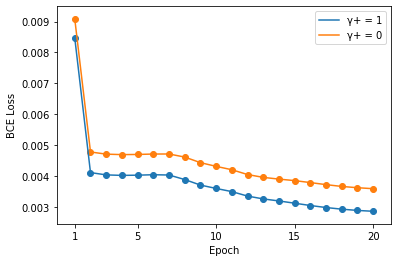
\includegraphics[width=\textwidth]{figures/supervised_approach/asl_pos_train_loss.png}
    \caption{Training loss}
    \label{fig:asl_pos_train_loss}
  \end{subfigure}
   \begin{subfigure}[t]{.5\textwidth}
    \centering
    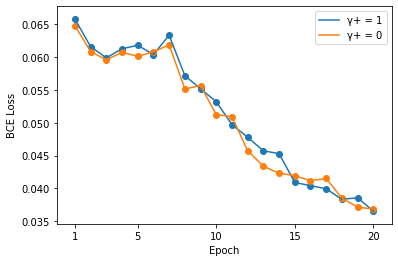
\includegraphics[width=\textwidth]{figures/supervised_approach/asl_pos_test_loss.png}
    \caption{Testing loss}
    \label{fig:asl_pos_test_loss}
  \end{subfigure}
  \caption{Test and training loss of models with different pos. gamma values.}
  \label{fig:asl_pos_train}
\end{figure}

\begin{figure}
  \begin{subfigure}[t]{.32\textwidth}
    \centering
    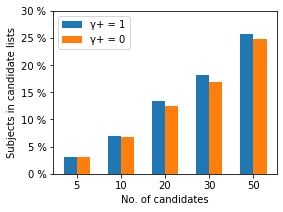
\includegraphics[width=\textwidth]{figures/supervised_approach/asl_pos_hw.png}
    \caption{Handwritten subjects}
    \label{fig:asl_pos_hw}
  \end{subfigure}
  \begin{subfigure}[t]{.32\textwidth}
    \centering
    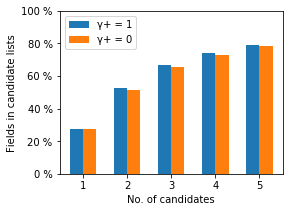
\includegraphics[width=\textwidth]{figures/supervised_approach/asl_pos_ddc.png}
    \caption{DDC subjects}
    \label{fig:asl_pos_ddc}
  \end{subfigure}
   \begin{subfigure}[t]{.32\textwidth}
    \centering
    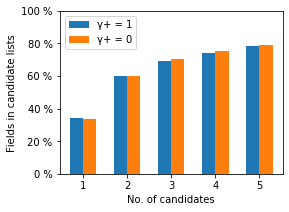
\includegraphics[width=\textwidth]{figures/supervised_approach/asl_pos_venue.png}
    \caption{Venues}
    \label{fig:asl_pos_venue}
  \end{subfigure}
  \caption{Model hit rate in the evaluation sets for different pos. gamma values.}
  \label{fig:asl_pos_eval}
\end{figure}

Now we experiment with the other parameter of ASL, $\gamma_+$. We train two models, with values zero and one for $\gamma_+$. Both models use the best result from the section above, $\gamma_-=2$. The authors state that setting $\gamma_+=0$ has shown to work well for most cases, which treats positive samples exactly as \acrshort{bce} does. This makes sense: given how rare positive samples are, we want to take full advantage of them.

On the other hand, as was explained in section \ref{hmc_asl}, setting $\gamma_+$ to a larger value than zero does not decrease the importance of all positive samples equally. It decreases the importance of positive samples whose corresponding model output is already very accurate, so the model can focus on those samples it still has trouble guessing correctly. Therefore, it is not obvious that setting $\gamma_+=0$ is optimal.

The results of the models on the evaluation datasets are shown in figure \ref{fig:asl_pos_eval}. Again, both models perform similarly in the venue and \acrshort{ddc} datasets. The difference between them can be seen in the handwritten dataset, where the model with the larger $\gamma_+$ value performs better. In contrast to the first experiment, where the training and test losses were very different, these models behaved similarly during training, as can be seen in figure \ref{fig:asl_pos_train}. We thus believe the results to be conclusive: the optimal parameters of \acrshort{asl} for our use case are $\gamma_+=1$ and $\gamma_-=2$.